\documentclass{beamer}

\newcommand{\rootpath}{../../}

\setbeamertemplate{navigation symbols}{}

\usetheme{Darmstadt}
\usecolortheme{whale}

\usepackage{ragged2e}
\usepackage{etoolbox}
\usepackage{lipsum}
\usepackage{algpseudocode}
\usepackage{algorithm}
\usepackage{multicol}
\usepackage{vwcol}
\usepackage{mdframed}
\usepackage{amsmath}
\usepackage{bm}


\apptocmd{\frame}{\justifying}{}{}
\beamersetuncovermixins{\opaqueness<1>{25}}{\opaqueness<2->{15}}

\setbeamertemplate{sidebar right}{}
\setbeamertemplate{footline}{
\hfill\usebeamertemplate***{navigation symbols}
\hspace{1cm}\insertframenumber{}/\inserttotalframenumber}

\begin{document}

\mdfsetup{
   middlelinecolor=red,
   middlelinewidth=0pt,
   backgroundcolor=red!20}



\title{Software Methodology at a Big Software Development Company}
\author{H\aa kan, Linnea, Dirk, Amir}
\institute[WASP]
{
 Wallenberg Autonomous Systems and Software Program\\
\medskip
}

\date{\today}
%================================%================================

\begin{frame}
\titlepage
\end{frame}

\begin{frame}\frametitle{Introduction of the Company}
\begin{itemize}
\item Product: Common Operation \& Maintenance (COM)
\item Process: Agile methods, hierarchical management, user/costumer in the loop,  
\item Organization: Large scale telecommunication company in Sweden
\end{itemize}
\end{frame}

\begin{frame}
  \frametitle{Methods}
  \begin{itemize}
  \item Surveys
   \item Case studies
   \item Experiments
  \end{itemize}
  For us, the method that suits best is a case study. \\
  "Case Study: a process or record of research into the development of a particular person, group, or situation over a period of time."
\end{frame}

\begin{frame}
  \frametitle{Methods}
  \begin{center}
    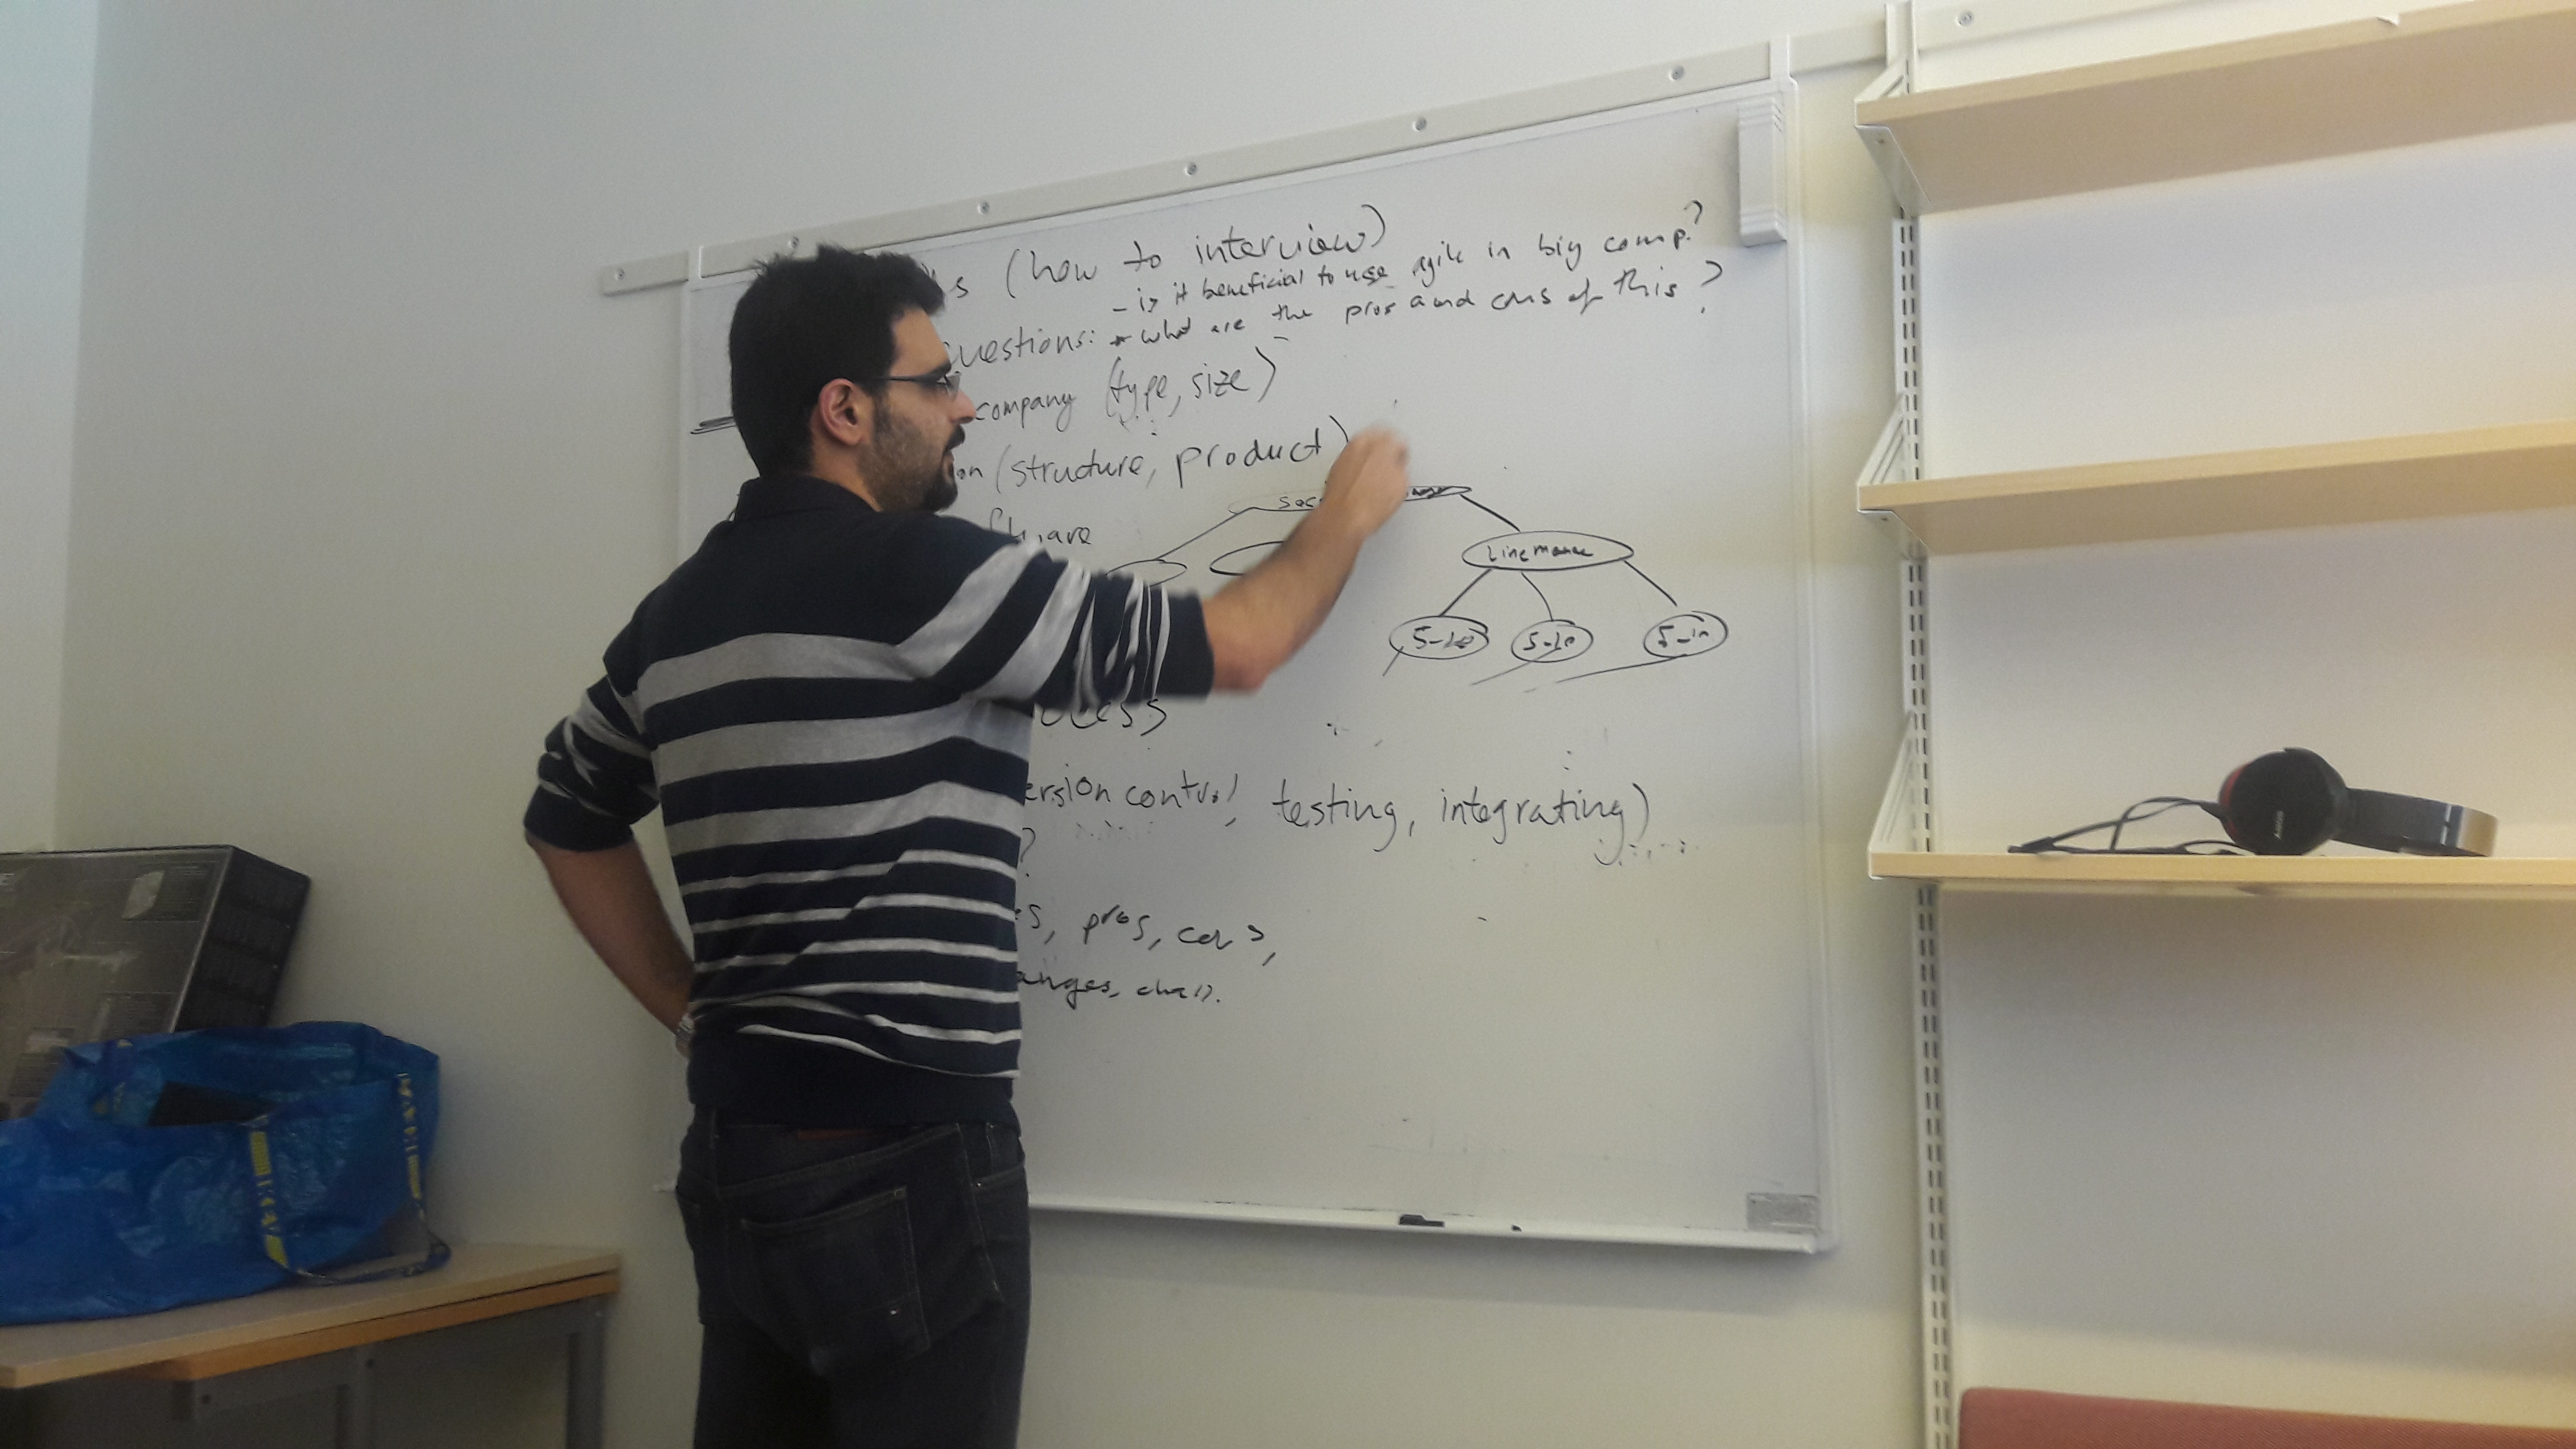
\includegraphics[width=1\textwidth]{figs/amir.jpg}
  \end{center}
\end{frame}

\begin{frame}
  \frametitle{Main questions}
  \begin{itemize}
  \item Is it beneficial to use agile in big companies?
  \item What are the pros and cons of this?
  \end{itemize}
\end{frame}

\begin{frame}
  \frametitle{Description of company}
  \begin{itemize}
  \item  Large scale telecommunication company in Sweden.
  \item Size: + 100 000 employees.
  \item Many different products
  \item Solutions ranging from Cloud services and Mobile Broadband to Network Design and Optimization.
  \item Services on software and infrastructure
  
  \end{itemize}
\end{frame}

\begin{frame}
  \frametitle{Organization}
  \begin{itemize}
  \item +25 000 in Research \& Development (R\&D).
  \item Different Product Development Unit -  break down to team with 5-10 members
    \begin{center}
    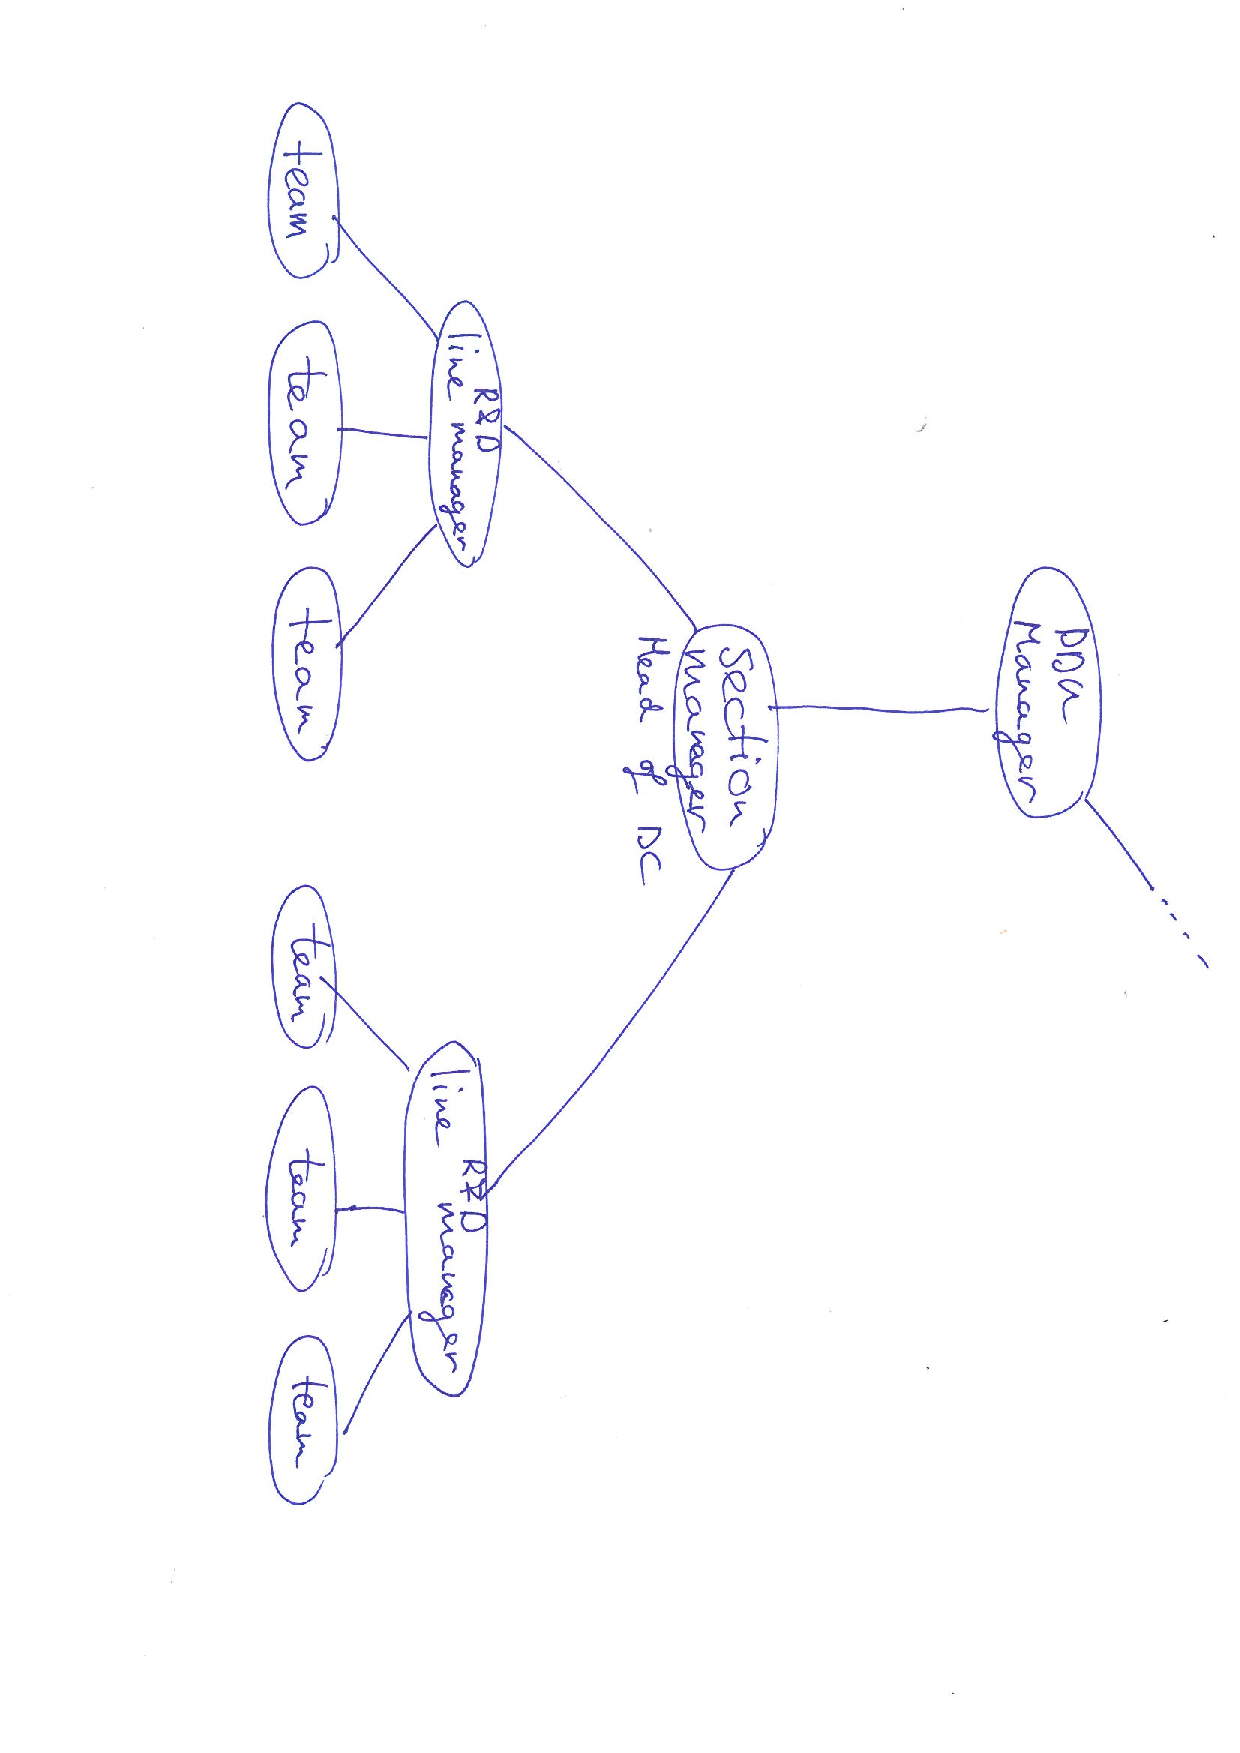
\includegraphics[width=0.5\textwidth, angle=90,origin=c]{figs/structure.pdf}
  \end{center}
  \item product
  \end{itemize}

\end{frame}

\begin{frame}
  \frametitle{Type of software}
  \begin{itemize}
  \item
  \end{itemize}
\end{frame}

\begin{frame}
  \frametitle{Workflow/process}
  \begin{itemize}
  \item The information is gathered from one team and the way they have been working 3 years ago 
  \item Note: This is not representative of how the company work 
  \begin{center}
    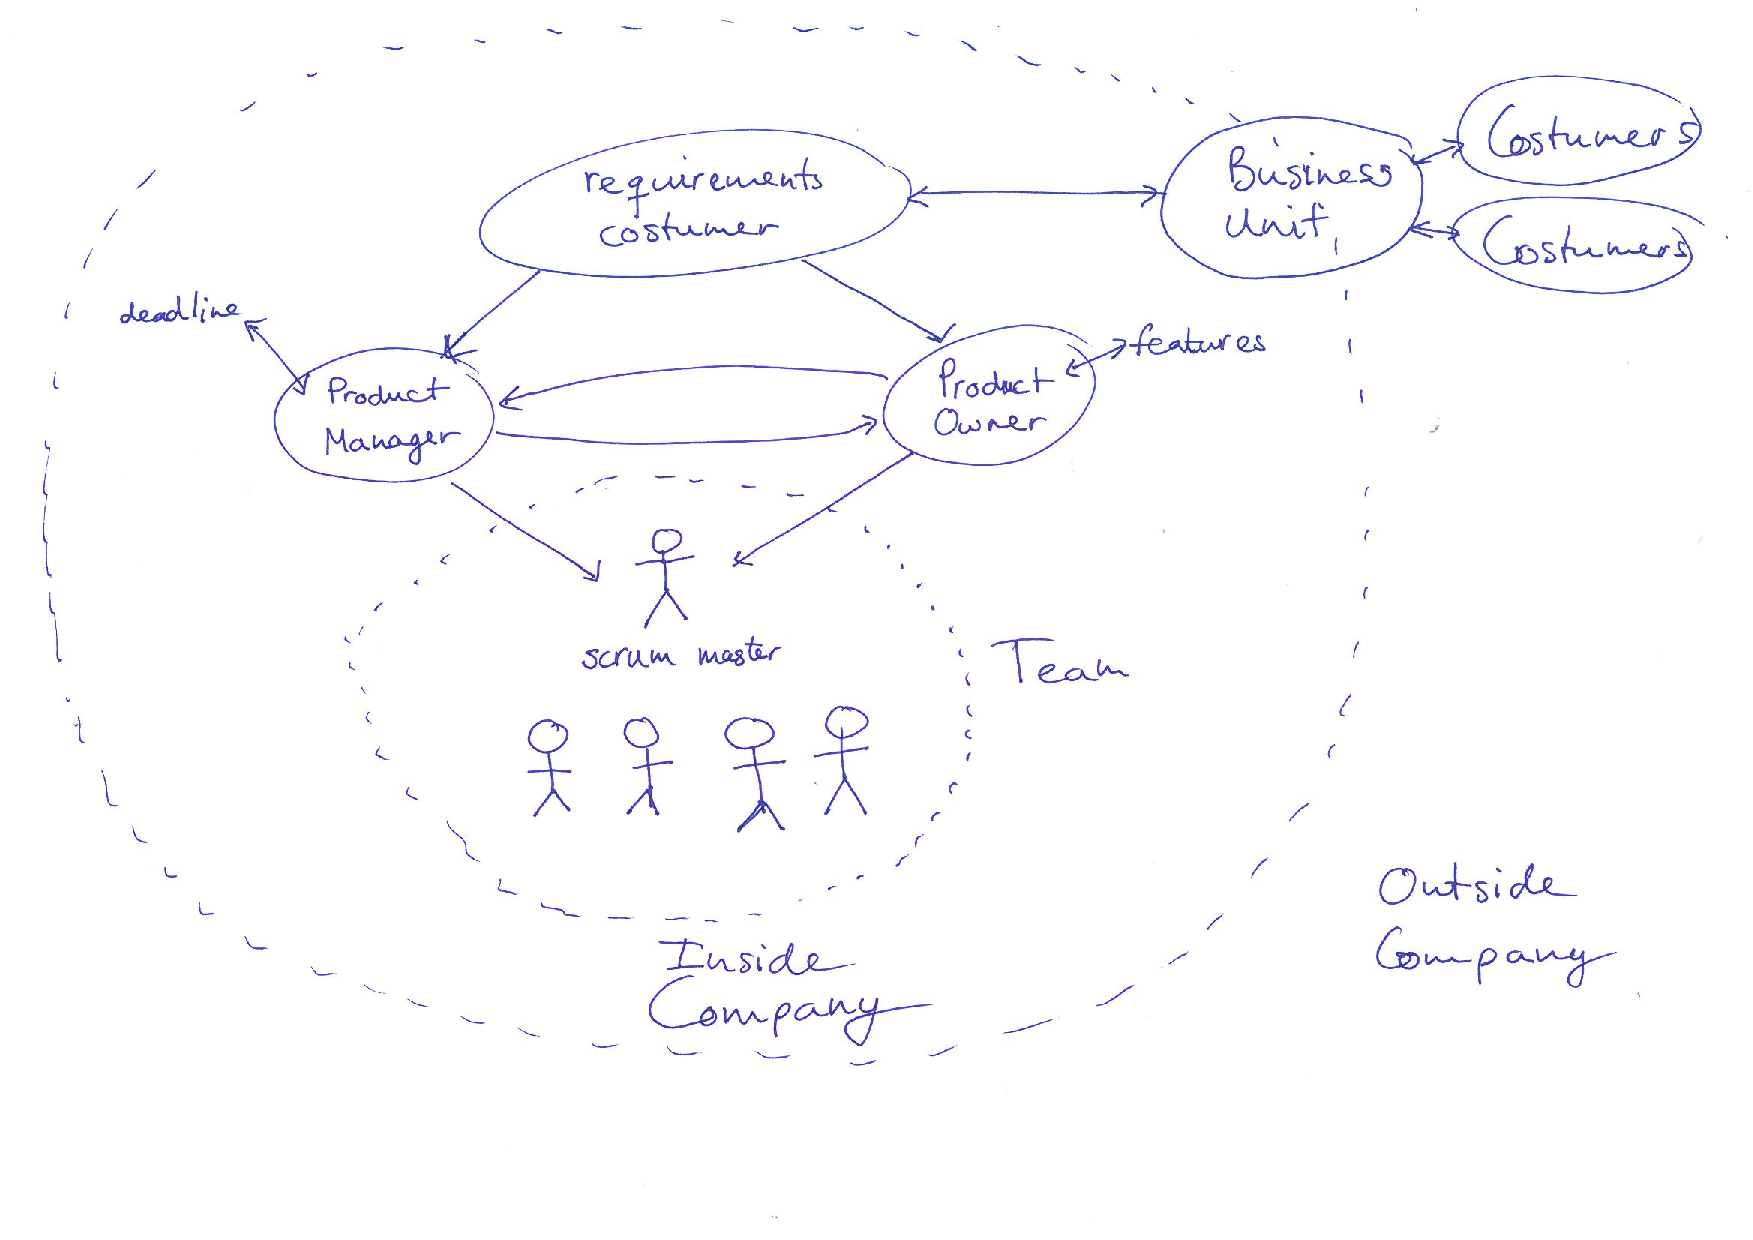
\includegraphics[width=1\textwidth]{figs/scrum_setup.pdf}
  \end{center}
  \end{itemize}
  
\end{frame}

\begin{frame}
  \frametitle{Tools}
  \begin{itemize}
  \item Version control: git, gerrit (code review), \url{https://www.gerritcodereview.com/}
  \item Testing: junit (unit
    testing in java)
  \item Integration: Jenkins
  \end{itemize}
\end{frame}

\begin{frame}
  \frametitle{Why scrum?}
  \begin{itemize}

  \item Waterfall is not working $\rightarrow$ Not able to release a
    product faster than a year at a time.
  \item Can update product with every sprint, every 3-4 weeks every
    team releases. Now the company releases the product 3-4 times per year.
    release a
  \item Company started implemented SCRUM a long time ago, still
    ongoing.
  \item Sprint defines the work for 3-4 weeks. None are allowed to
    interrupt you during this period.
  \item Provide greater efficiency.
  \item Stakeholder means different things in different contexts.
  \item stakeholders: make someone responseable for something?
    feauture to develop, stakeholder, other feature that are using
    your feature.
  \item Stakeholders come from interactions between features and teams.
  \item Cross competence team, within one teams solve difficult stuff.

  \end{itemize}
\end{frame}

\begin{frame}
  \frametitle{Challenges}
  \begin{itemize}
  \item Work bottom up. Good understanding at low level. 
  \item Higher management does not understand how agile and scrum works
  \item Hard to keep the customers in the loop
  \end{itemize}
\end{frame}

\begin{frame}
  \frametitle{Conclusions}
  \begin{itemize}
  \item Scrum has the potential to imrove work and efficiency at a company
  \item It might be difficult/take time to implement it at a large company
  \item Both programmers and management must be willing to change
  \end{itemize}
\end{frame}

\end{document}


%%% Local Variables:
%%% mode: latex
%%% TeX-master: t
%%% End:
